\chapter{Design of Data Structures}
\label{chap8}

Data Structures can be classified into - Memory Data Structures (In-core) and Disk Data Structures. 
\section{Disk Data Structures}
The Disk Data Structures are loaded to memory by the OS startup code and stored back when system terminates.
\subsection{\href{http://exposnitc.github.io/os_design-files/disk_ds.html#inode_table}{Inode Table}}

The Inode table is stored in the disk and has an entry for each file present in the disk. It consists of 32 entries. Thus eXpFS permits a maximum of 32 files.
\begin{figure}[ht]
\centering
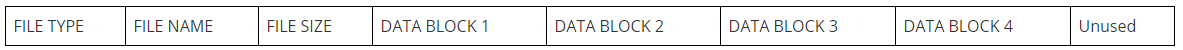
\includegraphics [scale=0.55]{figures/INODE.png}
\caption{\footnotesize Inode Table}
\end{figure}

\begin{itemize}
\item FILE TYPE (1 word) - specifies the type of the given file (ROOT indicated by 1 , DATA indicated by 2 or EXEC indicated by 3). 
\item FILE NAME (1 word) - Name of the file
\item FILE SIZE (1 word) - Size of the file. Maximum size for File = 2048 words
\item DATA BLOCK 1 to 4 (4 words) - each DATA BLOCK column stores the block number of a data block of the file. If a file does not use a particular DATA BLOCK , it is set to -1.
\item Unused (9 words) - All unused entries are set to -1.
\end{itemize}



\subsection{\href{http://exposnitc.github.io/os_design-files/disk_ds.html#disk_free_list}{Disk Free List}}

The Disk Free List consists of 512 entries each of size one word. For each block in the disk there is an entry in the Disk Free List which contains either 0 (free) or a number indicating the number of processes sharing the block.

\subsection{\href{http://exposnitc.github.io/os_design-files/disk_ds.html#root_file}{Root File}}

The Root File is stored in the disk and has an entry for each file present in the disk. It consists of 32 entries.

\begin{figure}[ht]
\centering
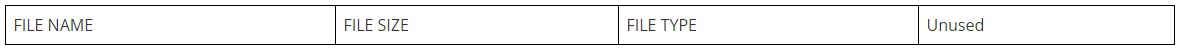
\includegraphics  [scale=0.55]{figures/ROOT.png}
\caption{\footnotesize Root File}
\end{figure}

\begin{itemize}

\item FILE NAME (1 word) - Name of the file
\item FILE SIZE (1 word) - Size of the file
\item FILE TYPE (1 word) - specifies the type of the given file (ROOT indicated by 1 , DATA indicated by 2 or EXEC indicated by 3).
\item Unused (5 words) - All unused entries are set to -1
\end{itemize}

\section {Memory Data Structures}

\subsection{\href{http://exposnitc.github.io/os_design-files/process_table.html}{Process Table}}

The Process Table (PT) contains an entry for each process present in the system. The entry is created when the process is created by a Fork system call. The maximum number of entries in PT (which is maximum number of processes allowed to exist at a single point of time in eXpOS) is 32.

\begin{figure}[ht]
\centering
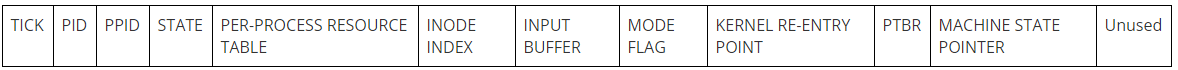
\includegraphics  [scale=0.55]{figures/pt.png}
\caption{\footnotesize Process Table}
\end{figure}

\begin {itemize}

\item TICK (1 word)- keeps track of how long the process was in memory. It has an initial value of 0 and is updated whenever the scheduler is called. TICK is reset to 0 when a process is swapped out or in.
\item PID (1 word) - process descriptor, set by Fork System Call.
\item PPID (1 word) - process descriptor of the parent process, set by Fork System Call.
\item STATE (2 words) - a two tuple that describes the current state of the process.
\item PER-PROCESS RESOURCE TABLE (16 words) - Per-Process Resource Table contains information about the files opened by the process as well as semaphores used by the process.
\item INODE INDEX (1 word)- Pointer to the Inode entry of the executable file, which was loaded into the process's address space.
\item INPUT BUFFER (1 word) - Buffer used to store the input read from the terminal. Whenever a word is read from the terminal, Terminal Interrupt Handler will store the word into this buffer.
\item MODE FLAG (1 word) - Used to indicate whether the process is executing in kernel (1) or user (0) mode. 
\item KERNEL RE-ENTRY POINT (1 word) - Contains the return address when a process voluntarily schedules out itself inside a blocking system call.
\item PTBR (1 word) - pointer to PER PROCESS PAGE TABLE.
\item MACHINE STATE POINTER(1 word) - pointer to a structure that gives the machine state when the process was last executed. The scheduler uses this structure to store the context of the process while scheduling. MACHINE STATE is architecture-dependent.
\item Unused (5 words)
\end {itemize}
Invalid entries are represented by -1.

\subsubsection {States}
The tuple can take the following values
\begin {itemize}
\item (RUNNING, \_ ): The process is in execution. This field is set by Scheduler when a process is scheduled.
\item (READY,  \_ ): The process is ready to be scheduled.
\item (WAIT\_PROCESS, WAIT\_PID): The process is waiting for a signal from another process whose PID is WAIT\_PID. This field is set by WAIT system call.
\item (WAIT\_FILE, FTENTRY): The process is blocked for a file whose file table entry index is FTENTRY.
\item (WAIT\_DISK,  \_ ): The process is blocked because of one of the following reasons:
\begin{enumerate}
\item It is waiting for disk to complete a disk-memory transfer operation it had initiated.
\item It wants to execute a disk transfer, but the disk is busy, handling a disk-memory transfer request issued by some other process.
\end{enumerate}
\item (WAIT\_SEMAPHORE, SEMID): The process is waiting for a semaphore (whose descriptor is SEMID) that was locked by some other process.
\item (WAIT\_MEM, \_): The process is blocked due to unavailability of memory pages.
\item (SWAPPED,  \_ ): The stack page of the process has been swapped out into disk.
\item (SWAPPED\_WAIT, WAIT\_PID): The stack page of a process which was in (WAIT\_PROCESS, WAIT\_PID) state has been swapped out into disk
\item (WAIT\_BUFFER, BUFFERID): The process is waiting for disk buffer of index BUFFERID to be unlocked.
\item (WAIT\_TERMINAL, \_ ): The process is waiting for Read from Terminal to be completed.
\end {itemize}
\\

\subsubsection {Machine State}
The OS scheduler can schedule out a process in execution and save its machine state here. Later, the scheduler can restore the machine state to start execution from where it had stopped. The initial values of this structure are fixed by the OS loader (or exec system call) and the values get updated whenever the process is preempted.
\begin{figure}[ht]
\centering
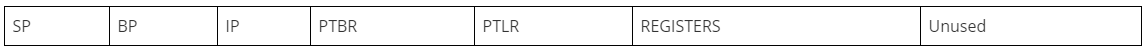
\includegraphics  [scale=0.55]{figures/ms.png}
\caption{\footnotesize Machine State}
\end{figure}

\begin {itemize}
\item SP (1 word)- Contents of Stack Pointer Register.
\item BP (1 word) - Contents of Base Pointer Register.
\item IP (1 word) - Contents of Instruction Pointer Register.
\item PTBR (1 word)- Contents of Page Table Base Register.
\item PTLR (1 word)- Contents of Page Table Length Register.
\item REGISTERS (24 words) - Machine registers.
\item Unused (3 words)
\end {itemize}

\subsubsection {Per Process Resource Table}

The Per-Process Resource Table has 8 entries and each entry is of 2 words. For every instance of file opened (or a semaphore acquired) by the process, it stores the index of the File Table (or Semaphore Table) entry for the file (or semaphore). In case of a file, the second word stores the LSEEK position of the open instance of that file. The LSEEK position indicates the location in the file where a word is read from or written to corresponding to the open instance of the file. In case of a semaphore, the second word is unused. File descriptor, returned by Open system call, is the index of the per-process resource table entry for that open instance of the file.
\begin{figure}[ht]
\centering
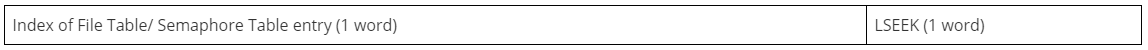
\includegraphics  [scale=0.55]{figures/prt.png}
\caption{\footnotesize Per Process Resource Table}
\end{figure}


\subsubsection {Per Process Page Table}
Each valid entry of the Per Process Page Table stores the physical page number corresponding to each logical (virtual) page associated with the process. The logical page number can vary from 0 to 7 for each process. Therefore, each process has 8 entries in the page table. 

Associated with each page table entry, typically auxiliary information is also stored. This is to store information like whether the process has write permission to the page, whether the page is dirty, referenced, valid etc. The exact details are architecture dependent.

\begin{figure}[ht]
\centering
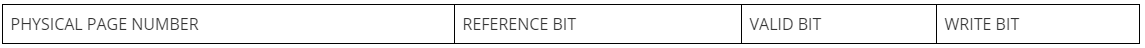
\includegraphics  [scale=0.55]{figures/pgt.png}
\caption{\footnotesize Per Process Page Table}
\end{figure}

\begin {itemize}
\item Reference bit - The reference bit for a page table entry is set to 0 by the OS when the page is loaded to memory and the page table initialized. When a page is accessed by a running process, the corresponding reference bit is set to 1 by the machine. This bit is used by the page replacement algorithm of the OS.
\item Valid bit - This bit is set to 1 by the OS when the physical page number field of a page table entry is valid (i.e, the page is loaded in memory). It is set to 0 if the entry is invalid. The OS expects the architecture to generate a page fault if any process attempts to access an invalid page.
\item Write bit - This bit is set to 1 by the OS if the page can be written and is set to 0 otherwise. The OS expects the architecture to generate an exception if any process attempts to modify a page whose write bit is not set.
\end {itemize}

\subsection{\href{http://exposnitc.github.io/os_design-files/mem_ds.html#file_table}{File Table}}
The File Table stores the information about all the files that are open while the OS is running. It consists of 32 entries. Thus, there can be at most 32 open files in the system at any time.
\begin{figure}[ht]
\centering
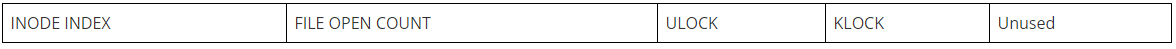
\includegraphics  [scale=0.55]{figures/ft.png}
\caption{\footnotesize File Table}
\end{figure}

\begin {itemize}
\item INODE INDEX (1 word) - specifies the index of the entry for the file in the Inode table.
\item FILE OPEN COUNT (1 word) - specifies the number of open instances of the file
\item ULOCK (1 word)- If the file was locked by a process using FLock system call, this field specifies the PID of the process, otherwise, it is set to -1.
\item KLOCK (1 word)- If the file is locked by the process inside a system call, this field specifies the PID of the process, otherwise, it is set to -1.
\item Unused (4 words)
\end {itemize}
All invalid entries are set to -1.

\subsection{\href{http://exposnitc.github.io/os_design-files/mem_ds.html#sem_table}{Semaphore Table}}

The Semaphore Table contains details about all the semaphores used by the processes. It consists of 32 entries. Thus, there can be at most 32 semaphores used in the system at any time. For every semaphore entry in the per-process resource table, there is a corresponding entry in the semaphore table.
\\
\begin{figure}[ht]
\centering
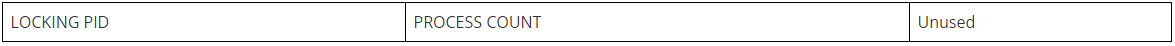
\includegraphics  [scale=0.55]{figures/st.png}
\caption{\footnotesize Semaphore Table}
\end{figure}

\begin {itemize}

\item LOCKING PID (1 word)- specifies the PID of the process which has locked the semaphore
\item PROCESS COUNT (1 word) - specifies the number of processes which are sharing the semaphore.
\item Unused (2 words)
\end {itemize}

All invalid entries are set to -1.

\subsection{\href{http://exposnitc.github.io/os_design-files/mem_ds.html#buffer_table}{Buffer Table}}
The buffer table is a data structure that stores the information regarding the disk block stored in each buffer. The present version of eXpOS sets MAX\_BUFFER = 4. Each buffer is identified by its index in the buffer table.
\begin{figure}[ht]
\centering
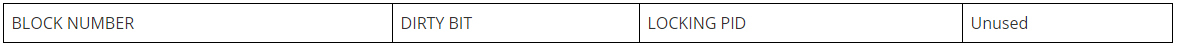
\includegraphics  [scale=0.55]{figures/bt.png}
\caption{\footnotesize Buffer Table}
\end{figure}
\begin {itemize}
\item BLOCK NUMBER (1 word) - specifies block number of the disk block which is currently stored in the buffer. It is set to -1 if the buffer does not contain any valid disk block.
\item DIRTY BIT (1 word) - specifies whether the block stored in the buffer has been modified. It is set to 0 when a disk block is loaded into the buffer and is set to 1 when modified by the Write System Call.
\item LOCKING PID (1 word) - specifies the PID of the process which has currently locked the buffer while executing a file system call.
\item Unused - (1 word)
\end {itemize}

Free entries are represented by -1 in all the fields.

\subsection{\href{http://exposnitc.github.io/os_design-files/mem_ds.html#ds_table}{Disk Status Table}}
The Disk Status Table keeps track of these disk-memory transfers. Every time a disk operation is invoked, the information regarding the operation like the disk block and the memory page involved, the process that invoked the operation and type of disk operation are stored in Disk Status Table by the OS.
\begin{figure}[ht]
\centering
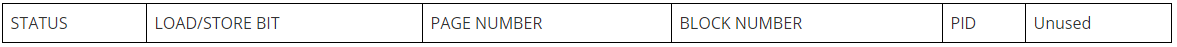
\includegraphics  [scale=0.55]{figures/ds.png}
\caption{\footnotesize Disk Status Table}
\end{figure}
\begin {itemize}

\item STATUS (1 word) - specifies whether the disk is free (indicated by 0) or busy (indicated by 1) handling a memory-disk transfer.
\item LOAD/STORE BIT (1 word) - specifies whether the operation being done on the device is a load (indicated by 0) or store (indicated by 1).
\item PAGE NUMBER (1 word) - specifies the memory page number involved in the disk transfer
\item BLOCK NUMBER (1 word) - specifies the disk block number involved in the disk transfer.
\item PID (1 word) - specifies the PID of the process which invoked the disk transfer. It is set to -PID if the disk transfer was initiated by the scheduler, to load/store a page of the process with identifier PID.
\item Unused (3 words)

\end {itemize}

\subsection{\href{http://exposnitc.github.io/os_design-files/mem_ds.html#ss_table}{System Status Table}}
It keeps the information about the number of free pages in memory, the number of processes blocked because memory is unavailable and, the number of processes in swapped state. 
\begin{figure}[ht]
\centering
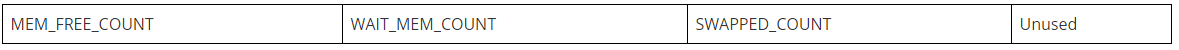
\includegraphics  [scale=0.55]{figures/sst.png}
\caption{\footnotesize System Status Table}
\end{figure}
\begin {itemize}
\item MEM\_FREE\_COUNT (1 word) - specifies the number of free pages available in memory.
\item WAIT\_MEM\_COUNT (1 word) - specifies the number of processes waiting for memory.
\item SWAPPED\_COUNT (1 word)- specifies the number of processes in (SWAPPED, \_ ) or (SWAPPED\_WAIT, \_ ) state.
\item Unused (1 word)
\end {itemize}

\subsection{\href{http://exposnitc.github.io/os_design-files/mem_ds.html#ts_table}{Terminal Status Table}}
The Terminal Status Table keeps track of the Read operations done on the terminal. Every time a Read system call is invoked on the terminal, the PID of the process that invoked the system call is stored in Terminal Status Table. 
\begin{figure}[ht]
\centering
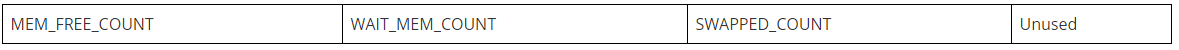
\includegraphics  [scale=0.55]{figures/ts.png}
\caption{\footnotesize Terminal Status Table}
\label{fig_1}
\end{figure}
\begin {itemize}

\item STATUS (1 word) - specifies whether the terminal is free or is being used by a process to read input. This field is initially set to 0. It is changed to 1 whenever terminal is busy. The Terminal Interrupt Handler sets back the status to 0 upon completion of Terminal Read.
\item PID (1 word) - specifies the PID of the process which is currently reading input from the terminal. This field is invalid when STATUS is 0.
\item Unused (2 words)
\end {itemize}
\subsection{\href{http://exposnitc.github.io/os_design-files/mem_ds.html#mem_free_list}{Memory Free List}}

The Memory free list is a data structure used for keeping track of used and unused pages in the memory. It consists of 128 entries and each entry is of size one word. Each entry of the free list contains either the value 0 indicating that the corresponding page in the memory is free (not allocated to any process) or contains the number of processes that are sharing the page. 
